\chapter{Decisions in Uncertainty}


\section{Bootstrapping}

\begin{enumerate}
    \item  The bootstrap provides a very general way to obtain a quantification of the uncertainty of an estimator.
    \hfill \cite{statistics/book/Statistics-for-Data-Scientists/Maurits-Kaptein}

    \item a larger sample decreases the variance of an estimator (i.e., the estimator becomes more precise).
    \hfill \cite{statistics/book/Statistics-for-Data-Scientists/Maurits-Kaptein}

    \item when estimating a population mean or difference in population means, we find that a smaller population variance leads to a smaller variance of the estimator.
    \hfill \cite{statistics/book/Statistics-for-Data-Scientists/Maurits-Kaptein}

    \item  The bootstrap has these exact same properties and is easy to carry out for many sample statistics; it provides a first entry into making decisions regarding populations based on sample data.
    \hfill \cite{statistics/book/Statistics-for-Data-Scientists/Maurits-Kaptein}

    \item  informally, it is quite clear that a large random sample and a relatively small variance of the estimator $\hat{\theta}$ should both increase our confidence regarding statements we can make about the population.
    \hfill \cite{statistics/book/Statistics-for-Data-Scientists/Maurits-Kaptein}

\end{enumerate}

\subsection{Basic Idea of Bootstrap}

\begin{enumerate}
    \item Given a (random) sample of size n from some population with distribution function $F_X$ , we frequently set out to obtain an estimate of a population parameter $\theta = T (x)$.
    \hfill \cite{statistics/book/Statistics-for-Data-Scientists/Maurits-Kaptein}

    \item Our point estimate of the parameter of interest is often what is called the “plug-in estimator” for $\theta$: $\hat{\theta} = T (x_1, \cdots , x_n )$; i.e., it is the statistic of interest calculated on the sample data $x_1, \cdots , x_n$ .
    \hfill \cite{statistics/book/Statistics-for-Data-Scientists/Maurits-Kaptein}

    \item we are interested in the distribution function of $\hat{\theta}$ over repeated samples.
    We are interested in $F_{\hat{\theta}}$ as it gives us information about the variability of our estimate over repeated samples.
    Depending on the statistic involved, the sampling plan, and the assumptions one is willing to make about $F_X$ or $f_X$ , we might be able to analytically derive $F_{\hat{\theta}}$.
    However, obtaining $F_{\hat{\theta}}$ in general (or properties thereof) can be challenging.
    \hfill \cite{statistics/book/Statistics-for-Data-Scientists/Maurits-Kaptein}

    \item The bootstrap addresses the problem of deriving $F_{\hat{\theta}}$ using the power of computer simulation.
    \hfill \cite{statistics/book/Statistics-for-Data-Scientists/Maurits-Kaptein}

    \item if we have a good estimate of the population distribution function $F_X$ , i.e., $\hat{F}_X$ , we can simply program a computer to obtain $M$ samples (by \textbf{simulation}) of size $n$ from $\hat{F}_X$ using the same sampling plan that we have used to collect our initial sample.
    If $\hat{F}_X$ is close to $F_X$ it does not really matter if we draw from $\hat{F}_X$ or $F_X$ .
    As long as our estimate of $\hat{F}_X$ is close to the true $F_X$ , our samples of $\hat{F}_{\hat{\theta}}$ can be used to approximate properties of $F_{\hat{\theta}}$
    \hfill \cite{statistics/book/Statistics-for-Data-Scientists/Maurits-Kaptein}

    \item On each sample $m = 1, \cdots , M$ we can subsequently compute the statistic of interest, $\hat{\theta}^{(1)} , \cdots , \hat{\theta}^{(M)}$ which themselves serve as approximate samples from $F_{\hat{\theta}}$ (approximate as we are using $\hat{F}_X $, and thus we obtain samples from $\hat{F}_{\hat{\theta}}$).
    \hfill \cite{statistics/book/Statistics-for-Data-Scientists/Maurits-Kaptein}

    \item standard error of a statistic can simply be computed by computing the standard deviation of the M samples of the statistic of interest
    $
        \hat{SE}(\hat{\theta})
        = \sqrt{\dfrac{\dsum^M_{m=1} \dParenBrac{\hat{\theta}^{(m)}-\bar{\theta}}^2}{M-1}}
    $
    where
    $
        \bar{\theta} = \dfrac{1}{M} \dsum^M_{m=1} \hat{\theta}^{(m)}
    $
    \hfill \cite{statistics/book/Statistics-for-Data-Scientists/Maurits-Kaptein}

    \item we are interested in the variability of our estimator over differently obtained samples, we should adopt our bootstrapping procedure accordingly.
    \hfill \cite{statistics/book/Statistics-for-Data-Scientists/Maurits-Kaptein}

    \item Although the bootstrap is appealing as it allows one to quantify the uncertainty for virtually any statistic—by simply replacing tedious analytical work with simple computer operations—one should always be careful: for complex sampling schemes and complex population distributions, $\hat{F}_X$ , or the resulting $M$ bootstrap samples of the statistic of interest, might not provide a good quantification of the uncertainty associated with $\hat{\theta}$.
    \hfill \cite{statistics/book/Statistics-for-Data-Scientists/Maurits-Kaptein}

    \item We can use $\hat{F}_X$ , in combination with computer simulation, to generate bootstrap samples $m = 1, \cdots , M$ and compute $\hat{\theta}(m)$ for arbitrary statistics $T $.
    \hfill \cite{statistics/book/Statistics-for-Data-Scientists/Maurits-Kaptein}

    \item \textbf{Steps}:
    \begin{enumerate}
        \item we estimate $F_X$ based using our sample $x_1, \cdots , x_n$ . This gives us $\hat{F}_X $.
        \hfill \cite{statistics/book/Statistics-for-Data-Scientists/Maurits-Kaptein}

        \item we obtain $M$ random samples from $\hat{F}_X$ (each of size $n$), on which we computed our bootstrap estimates of the statistic of interest $\hat{\theta}^{(1)} , \cdots, \hat{\theta}^{(M)}$ which we regard as (approximate) samples from $F_{\hat{\theta}}$.
        \hfill \cite{statistics/book/Statistics-for-Data-Scientists/Maurits-Kaptein}
    \end{enumerate}

    \item \textbf{Disadvantages}:
    \begin{enumerate}
        \item it might be the case that $\hat{F}_X$ is a very poor estimate of $F_X$ .
        This is often the case when $n$ is small, but it might also be caused by the fact that the original sample $x_1, \cdots , x_n$ is not obtained through simple random sampling (resampling with replacement).
        If the latter is the case, the sampling scheme that was used should be taken into consideration when computing $\hat{F}_X$.
        \hfill \cite{statistics/book/Statistics-for-Data-Scientists/Maurits-Kaptein}

        \item the sampling scheme implemented in the second step (resampling step) should mimic the sampling scheme that was originally used: if the $M$ bootstrap samples are generated using a different sampling scheme than the sampling scheme of interest, $F_{\hat{\theta}}$ might not be properly approximated by the M bootstrap samples.
        \hfill \cite{statistics/book/Statistics-for-Data-Scientists/Maurits-Kaptein}

        \item While the bootstrap provides an easy way of quantifying uncertainty that we can use to make decisions, it is hard in general to make statements about the \textbf{quality} of these decisions.
        \hfill \cite{statistics/book/Statistics-for-Data-Scientists/Maurits-Kaptein}
    \end{enumerate}

\subsubsection{Non-Parametric Bootstrap}

    \item no parametric assumptions regarding $F_X$ are made in this procedure
    \hfill \cite{statistics/book/Statistics-for-Data-Scientists/Maurits-Kaptein}

    \item  The simplest bootstrap approach for obtaining $\hat{F}_X$ is to simply use the empirical distribution function: the original samples $x_1, \cdots , x_n$ in our sample can be used to construct a discrete approximation of $F_X$ by simply giving each unique value $v_i$ in $x_1, \cdots , x_n$ probability $\dfrac{1}{n}$ .
    \hfill \cite{statistics/book/Statistics-for-Data-Scientists/Maurits-Kaptein}

\subsubsection{Parametric Bootstrap}

    \item in the parametric bootstrap $\hat{F}_X$ is assumed to be of a certain form (e.g., it is assumed to be normal), and plug-in estimates for its parameters (e.g., $\hat{\mu}$ and $\hat{\sigma}^2$ in the normal case) are used to estimate $F_X$ .
    \hfill \cite{statistics/book/Statistics-for-Data-Scientists/Maurits-Kaptein}

    \item If the assumptions are correct, the parametric bootstrap is preferable over the non-parametric bootstrap.
    \hfill \cite{statistics/book/Statistics-for-Data-Scientists/Maurits-Kaptein}

\end{enumerate}






\section{Hypothesis testing}

\begin{enumerate}
    % \item  make binary decisions
    % \hfill \cite{statistics/book/Statistics-for-Data-Scientists/Maurits-Kaptein}

    \item \textbf{Test Statistics} ($t$): A single number that summarizes the sample data used to conduct the test hypothesis.
    \hfill \cite{ctl.unm.edu/assets/docs/resources/hypothesis-testing-sheet.pdf}

    \item $p$-\textbf{value}: Probability of observing a test statistics.
    \hfill \cite{ctl.unm.edu/assets/docs/resources/hypothesis-testing-sheet.pdf}


    \item without making any assumptions regarding the sampling process and/or the population distributions involved, it is practically impossible to say anything about the population based on sample data with full certainty.
    \hfill \cite{statistics/book/Statistics-for-Data-Scientists/Maurits-Kaptein}

    \item Hypothesis testing provides a method for making binary decisions that, in many instances, does give us clear quantitative statements about the quality of the decisions we make.
    \hfill \cite{statistics/book/Statistics-for-Data-Scientists/Maurits-Kaptein}

    \item Within hypothesis testing the general setup is as follows: we state our decision problem as a choice between two competing hypotheses regarding the population, often called the \textbf{null hypothesis} $H_0 $, and the \textbf{alternative hypothesis} $H_a $.
    Given that $H_0$ and $H_a$ are complementary, one of the two \textbf{must} be true in the population.
    \hfill \cite{statistics/book/Statistics-for-Data-Scientists/Maurits-Kaptein}
    \begin{enumerate}
        \item \textbf{Null Hypothesis} ($H_0$): A statement of no change and is 0 assumed true until evidence indicates otherwise.
        \hfill \cite{ctl.unm.edu/assets/docs/resources/hypothesis-testing-sheet.pdf}

        \item \textbf{Alternate Hypothesis} ($H_a$): A statement that the researcher is trying to find evidence to support
        \hfill \cite{ctl.unm.edu/assets/docs/resources/hypothesis-testing-sheet.pdf}
    \end{enumerate}

    \item The subsequent rationale of hypothesis testing is that we assume that the null hypothesis is true and that we gather \textbf{sufficient evidence} to demonstrate that it is not true.
    It defines sufficient evidence such that the probability of making a type 1 error is \textbf{at most} $\alpha$.
    The level $\alpha$ is called the \textbf{significance level} and it is the maximal allowable probability of rejecting the null hypothesis when the null hypothesis is actually true.
     It is often set equal to a value of $\alpha = 0.05$ or $\alpha = 0.01$.
    \hfill \cite{statistics/book/Statistics-for-Data-Scientists/Maurits-Kaptein}

    \item  Thus the \textbf{goal} of hypothesis testing is to \textbf{reject the null hypothesis} on the basis of sufficient and well-collected data.
    We will decide that either $H_0$ is rejected (thus $H_a$ must be true) or is not rejected (thus there is no or not enough evidence to demonstrate that $H_0$ is false).
    \hfill \cite{statistics/book/Statistics-for-Data-Scientists/Maurits-Kaptein}


\begin{figure}[H]
    \centering
    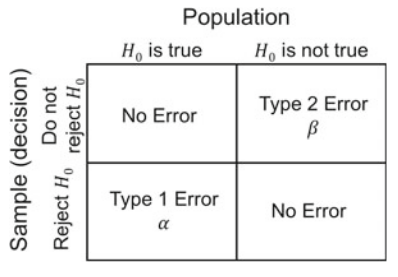
\includegraphics[
        width=\linewidth,
        height=5cm,
        keepaspectratio,
    ]{images/statistics/hypothesis-testing-errors.png}
    \caption{
        Types of errors in hypothesis testing
        \cite{statistics/book/Statistics-for-Data-Scientists/Maurits-Kaptein}
    }
\end{figure}

    \item 4 situations:
    \begin{enumerate}
        \item {[\textbf{true positive}]} we do not reject $H_0$ when $H_0$ is true in the population
        \hfill \cite{statistics/book/Statistics-for-Data-Scientists/Maurits-Kaptein}

        \item {[\textbf{true negative}]} we reject $H_0 $, and subsequently accept $H_a $, when $H_a$ is true in the population
        \hfill \cite{statistics/book/Statistics-for-Data-Scientists/Maurits-Kaptein}

        \item {[\textbf{false positive}]} we reject $H_0$ while in reality it is true, aka false positive or type 1 error.
        The probability of a type 1 error is associated with the level $\alpha$.
        The $\alpha$ is used as a maximal allowable type 1 error for a decision rule.
        \hfill \cite{statistics/book/Statistics-for-Data-Scientists/Maurits-Kaptein}

        \item {[\textbf{false negative}]} we do not reject $H_0$ , while in actuality $H_a$ is true, aka type 2 error.
        The probability of a type 2 error is associated with the level $\beta$.
        The value $\beta$ is used a maximal allowable type 2 error.
        One minus the type 2 error ($1-\beta$) is called the \textbf{power} of the binary decision rule.
        It indicates how likely the null hypothesis is rejected when the alternative hypothesis is true.
        \hfill \cite{statistics/book/Statistics-for-Data-Scientists/Maurits-Kaptein}
    \end{enumerate}

    \item it is easy to create a decision procedure that has a type 1 error probability equal to zero:
    if we simply never reject $H_0$ —in this case basically we state that there is never sufficient evidence to reject $H_0$ —we will never make a type 1 error.
    While this decision procedure does control the type 1 error, it is clearly not very useful, as the power of this decision rule is zero: we never accept the alternative hypothesis when it is true.
    \hfill \cite{statistics/book/Statistics-for-Data-Scientists/Maurits-Kaptein}

    \item the procedure of hypothesis testing aims to be less conservative (e.g., it will reject the null hypothesis sometimes but not too often when it would be true).
    \hfill \cite{statistics/book/Statistics-for-Data-Scientists/Maurits-Kaptein}

    \item \textbf{One tailed test}: Test statistics falls into one specified tail of its sampling distribution
    \hfill \cite{ctl.unm.edu/assets/docs/resources/hypothesis-testing-sheet.pdf}

    \item \textbf{Two tailed test}: Test statistics can falling into either tail of its sampling distribution
    \hfill \cite{ctl.unm.edu/assets/docs/resources/hypothesis-testing-sheet.pdf}

    \item Steps to Significance Testing:
    \hfill \cite{ctl.unm.edu/assets/docs/resources/hypothesis-testing-sheet.pdf}
    \begin{enumerate}
        \item Define $H_0$ and $H_a$
        \hfill \cite{ctl.unm.edu/assets/docs/resources/hypothesis-testing-sheet.pdf}

        \item Identify test, $\alpha$, find critical value, test statistics
        \hfill \cite{ctl.unm.edu/assets/docs/resources/hypothesis-testing-sheet.pdf}

        \item Construct acceptance/rejection regions
        \hfill \cite{ctl.unm.edu/assets/docs/resources/hypothesis-testing-sheet.pdf}

        \item Calculate test statistics
        \hfill \cite{ctl.unm.edu/assets/docs/resources/hypothesis-testing-sheet.pdf}

        \begin{enumerate}
            \item Critical value approach: Determine critical region
            \hfill \cite{ctl.unm.edu/assets/docs/resources/hypothesis-testing-sheet.pdf}

            \item p-value approach: Calculate p-value
            \hfill \cite{ctl.unm.edu/assets/docs/resources/hypothesis-testing-sheet.pdf}
        \end{enumerate}

        \item Retain or reject the hypothesis
        \hfill \cite{ctl.unm.edu/assets/docs/resources/hypothesis-testing-sheet.pdf}
    \end{enumerate}

    \item \textbf{Choosing a Statistical Test}:

\begin{figure}[H]
    \centering
    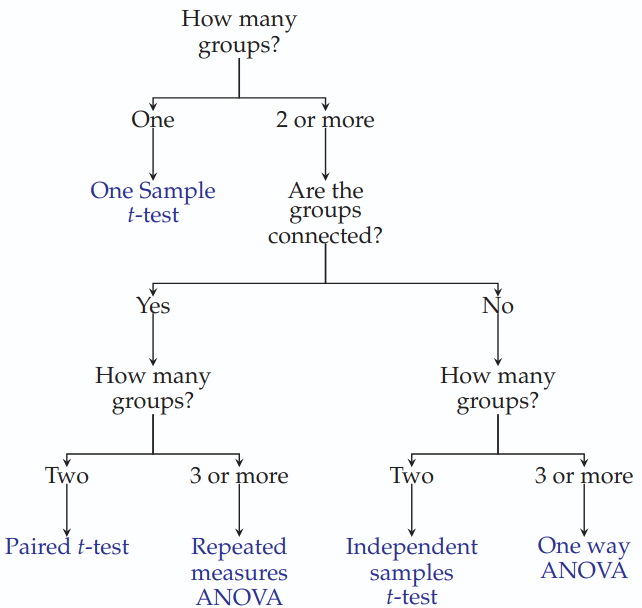
\includegraphics[
        width=\linewidth,
        height=7cm,
        keepaspectratio,
    ]{images/statistics/hypothesis-testing-desicion-tree.png}
    \caption{
        Choosing a Statistical Test: Decision Tree
        \cite{ctl.unm.edu/assets/docs/resources/hypothesis-testing-sheet.pdf}
    }
\end{figure}

    \begin{enumerate}
        \item Categorical Data: Use Chi Square
        \hfill \cite{ctl.unm.edu/assets/docs/resources/hypothesis-testing-sheet.pdf}

        \item Sample size ($n$):
        \begin{enumerate}
            \item $n < 30$ and Population Variance is unknown - t-test
            \hfill \cite{ctl.unm.edu/assets/docs/resources/hypothesis-testing-sheet.pdf}

            \item $n < 30$ and Population Variance is known - z-test
            \hfill \cite{ctl.unm.edu/assets/docs/resources/hypothesis-testing-sheet.pdf}

            \item $n > 30$ - z-test or t-test
            \hfill \cite{ctl.unm.edu/assets/docs/resources/hypothesis-testing-sheet.pdf}
        \end{enumerate}
    \end{enumerate}

    \item The z-test heavily depends on asymptotic theory and therefore requires \textbf{large sample sizes}.
    \hfill \cite{statistics/book/Statistics-for-Data-Scientists/Maurits-Kaptein}

    \item the t-test can be used for small sample sizes but under the strict assumption of having collected data from a \textbf{normal distribution}.
    \hfill \cite{statistics/book/Statistics-for-Data-Scientists/Maurits-Kaptein}

    \item Alternative approaches for the z-test and t-test have been developed that require fewer or no assumptions. These tests are referred to as \textbf{non-parametric tests}.
    \hfill \cite{statistics/book/Statistics-for-Data-Scientists/Maurits-Kaptein}

    \item The term \textbf{heteroskedasticity} refers to differences in variation or variability. 
    In hypothesis testing this is often translated to a hypothesis on the variances or standard deviations from two different populations, as we described for the two samples t-test.
    Under the assumption of normality the most efficient test statistic (F-test) is based on a ratio of the two sample variances, but under non-normal data an alternative approach (Levene’s test) has been suggested. 
    \hfill \cite{statistics/book/Statistics-for-Data-Scientists/Maurits-Kaptein}

    \item The common practice of testing the (two-sided) null hypothesis has a few \textbf{drawbacks}.
    \hfill \cite{statistics/book/Statistics-for-Data-Scientists/Maurits-Kaptein}
    \begin{enumerate}
        \item For (extremely) large samples we will almost always reject the null hypothesis. 
        This might not be desirable, as rejecting the null hypothesis in such cases does not actually imply that the (e.g.,) difference in means of interest is indeed large. 
        \hfill \cite{statistics/book/Statistics-for-Data-Scientists/Maurits-Kaptein}
        
        \item Not rejecting the null hypothesis $H_0 : \mu( f ) = \mu_0$ is no proof that the null hypothesis is true.
        It is very easy not to reject the null hypothesis: you just need to collect as little information as possible. 
        If we would collect only a few observations the confidence interval would be very wide and the value $\mu_0$ is likely to fall inside this wide confidence interval, but this does not guarantee that $\mu( f ) = \mu_0$ or even close to it.
        \hfill \cite{statistics/book/Statistics-for-Data-Scientists/Maurits-Kaptein}
    \end{enumerate}
    One way of dealing with these two issues on hypothesis testing is to reduce the significance level $\alpha$ to a much lower value than the commonly used $\alpha = 0.05$. 
    We may use $\alpha = 0.001$ or even $\alpha = 0.0001$ to make the hypothesis statements more confident than just $95\%$. 
    \hfill \cite{statistics/book/Statistics-for-Data-Scientists/Maurits-Kaptein}
\end{enumerate}


\begin{figure}[H]
    \centering
    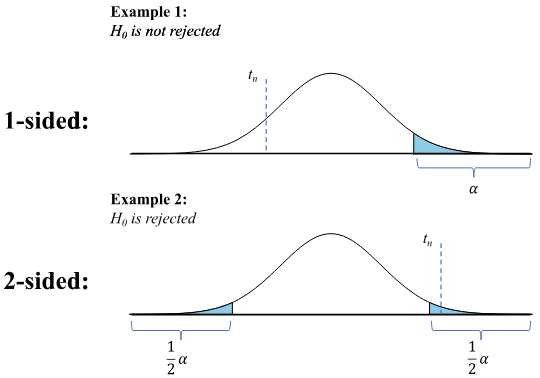
\includegraphics[
        width=\linewidth,
        height=5.5cm,
        keepaspectratio,
    ]{images/statistics/one-sided_two-sided_t-test.png}
\end{figure}

The difference between one-sided and two-sided tests.
In both cases $H_0$ is not rejected if the observed test statistic $t_n$ falls outside of the rejection region $\alpha$.
However, for a one-sided test (top) the rejection region is located on one tail of the distribution (the blue area denoted $\alpha$).
Hence, only if $t_n > z_{1-\alpha}$ (in this case), and sufficiently large to fall within the rejection region, is $H_0$ rejected.
For a two-sided test the rejection region is split over the two tails of the distribution: hence $H_0$ can be rejected if $t_n$ is either sufficiently small or sufficiently large.
Finally, note that if $t_n > z_{1-\alpha}$—if this is the direction of the one-sided test—a one-sided test might reject $H_0 $, whereas the same $t_n$ might not lead to a rejection in the two-sided case, because the critical value for the two-sided test is larger than for the one-sided test
\hfill \cite{statistics/book/Statistics-for-Data-Scientists/Maurits-Kaptein}

















\subsection{The One-Sided $z$-Test for a Single Mean ($H_0:\mu(f) \leq \mu_0$)}

\begin{enumerate}
    \item hypothesis on the population mean: $H_0 : \mu( f ) \leq \mu_0$ versus $H_a : \mu( f ) > \mu_0 $.
    \hfill \cite{statistics/book/Statistics-for-Data-Scientists/Maurits-Kaptein}

    \item we assume that the sample is large enough to be able to use the normal distribution function as an approximation to the distribution function of the statistic that we are using to make a decision about the null hypothesis
    \hfill \cite{statistics/book/Statistics-for-Data-Scientists/Maurits-Kaptein}

    \item Let’s assume that we have collected a random sample $Y_1 , Y_2, \cdots , Y_n$ from the population.
    We may estimate the population mean $\mu ( f )$ with the sample average $\bar{Y}$ .
    \hfill \cite{statistics/book/Statistics-for-Data-Scientists/Maurits-Kaptein}

    \item when $\bar{Y}$ is smaller or equal to $\mu_0$ the random variable $\bar{Y}$ seems to be in line with the null hypothesis $H_0 : \mu( f ) \leq \mu_0$ .
    In other words, there is no evidence that the \textbf{null hypothesis is false}.
    \hfill \cite{statistics/book/Statistics-for-Data-Scientists/Maurits-Kaptein}

    \item Although the random variable does not suggest any conflict with the null hypothesis $H_0 : \mu( f ) \leq \mu_0 $, it \textbf{does not guarantee} that $\mu( f ) \leq \mu_0$ either.
    \hfill \cite{statistics/book/Statistics-for-Data-Scientists/Maurits-Kaptein}

    \item If the population mean $\mu( f )$ were somewhat larger than $\mu_0 $, it might not be completely unlikely to observe a sample average still below $\mu_0$ due to the sampling (a type 2 error).
    \hfill \cite{statistics/book/Statistics-for-Data-Scientists/Maurits-Kaptein}

    \item When $\bar{Y}$ is larger than $\mu_0 $, we might start to believe that the null hypothesis is incorrect.
    However, when $\bar{Y}$ is just a little higher than $\mu_0$ this might not be very unlikely either, even when $\mu( f ) \leq \mu_0$ .
    \hfill \cite{statistics/book/Statistics-for-Data-Scientists/Maurits-Kaptein}

    \item For instance, for any symmetric $f$ at $\mu( f ) = \mu_0 $, the probability that $\bar{Y}$ is larger than $\mu_0$ is equal to $0.5$.
    Only when the sample average $\bar{Y}$ is substantially larger—thus when there is sufficient evidence—than $\bar{Y}$ would we start to indicate that the null hypothesis $H_0 : \mu( f ) \leq \mu_0$ is unlikely to be true (although a type 1 error could be made here).
    \hfill \cite{statistics/book/Statistics-for-Data-Scientists/Maurits-Kaptein}

    \item we want to find a criterion for the average $\bar{Y}$ such that the average can only be larger than this criterion with a probability that is at most equal to $\alpha$ when the null hypothesis is true.
    If we assume that this criterion is equal to $\mu_0 + \delta$, with $\delta > 0$, then the probability that $\bar{Y}$ is larger than $\mu_0 + \delta$ is given by
    \hfill \cite{statistics/book/Statistics-for-Data-Scientists/Maurits-Kaptein}
    \\[0.3cm]
    .\hfill
    $
        P( \bar{Y} > \mu _0 + \delta)
        = P\dParenBrac{\dfrac{ ( \bar{Y} - \mu ( f ))}{\sigma( f )/\sqrt{n}} > \dfrac{\mu _0 - \mu ( f ) + \delta}{\sigma/\sqrt{n}}}
        \approx 1 - \Phi\dParenBrac{\dfrac{\mu _0 - \mu ( f ) + \delta}{\sigma( f )/\sqrt{n}}}
    $
    \hfill \cite{statistics/book/Statistics-for-Data-Scientists/Maurits-Kaptein}
    \\[0.3cm]
    where $\Phi$ is the standard normal PDF.
    \hfill \cite{statistics/book/Statistics-for-Data-Scientists/Maurits-Kaptein}

    \item Under the null hypothesis $H_0 : \mu( f ) \leq \mu_0$ this probability is the type 1 error and it is maximized when $\mu( f ) = \mu_0$ .
    \hfill \cite{statistics/book/Statistics-for-Data-Scientists/Maurits-Kaptein}

    \item if we deliberately set $\mu( f ) = \mu_0$ to maximize the type 1 error, the probability $P ( \bar{Y} > \mu_0 + \delta)$ is given by $1 - \Phi(\delta\sqrt{n}/\sigma)$.
    \hfill \cite{statistics/book/Statistics-for-Data-Scientists/Maurits-Kaptein}

    \item When we choose $\delta$ equal to $\delta = \dfrac{z_{1-\alpha} \sigma( f )}{\sqrt{n}}$, the probability becomes $P ( \bar{Y} > \mu_0 + \delta) \approx \alpha$.
    When $\bar{Y} > \mu_0 + \dfrac{z_{1 - \alpha} \sigma( f )}{\sqrt{n}}$ the probability of rejecting the null hypothesis is at most $\alpha$—and hence we have defined sufficient evidence by the criterion $\mu0 + \dfrac{z_{1 - \alpha} \sigma( f )}{\sqrt{n}}$ for the null hypothesis $H_0 : \mu( f ) \leq \mu_0$ using the statistic $\bar{Y} $.
    \hfill \cite{statistics/book/Statistics-for-Data-Scientists/Maurits-Kaptein}

    \item The null hypothesis could still be true, but that it is just bad luck to have observed such an unlikely large average under the null hypothesis.
    However, we know that this probability of having bad luck is less than or equal to $\alpha$ and therefore we accept making this potential type 1 error.
    \hfill \cite{statistics/book/Statistics-for-Data-Scientists/Maurits-Kaptein}

    \item we cannot use the criterion ¯$Y > \mu_0 + \dfrac{z_{1-\alpha} \sigma( f )}{\sqrt{n}}$ directly, as it depends on the population standard deviation $\sigma( f )$, which is generally not known.
    We could estimate $\sigma( f )$ using sample standard deviation $S = \sqrt{\dfrac{1}{n-1} \dsum^n_{i=1} (Y_i - \bar{Y} )^2}$
    \hfill \cite{statistics/book/Statistics-for-Data-Scientists/Maurits-Kaptein}

    \item If the sample size is large enough, the probability $P\dParenBrac{\bar{Y} > \mu_0 + \dfrac{z_{1-\alpha} S}{\sqrt{n}}}$ would still be close to $\alpha$.
    When the sample size is large enough, we may reject the null hypothesis in practice when $\bar{Y} > \mu_0 + \dfrac{z_{1-\alpha} S}{\sqrt{n}}$ or in other words when the \textbf{asymptotic test statistic} $T_n = \dfrac{\bar{Y} - \mu_0}{S/\sqrt{n}}$ is larger than $z_{1-\alpha}$.
    \hfill \cite{statistics/book/Statistics-for-Data-Scientists/Maurits-Kaptein}

    \item For large sample sizes n, the null hypothesis $H_0 : \mu( f ) \leq \mu_0$ is tested with test statistic $T_n = \dfrac{\bar{Y} - \mu_0}{S/\sqrt{n}}$ and the null hypothesis is rejected with significance level $\alpha$ when the test statistic is larger than the critical value $z_{1-\alpha}$.
    \hfill \cite{statistics/book/Statistics-for-Data-Scientists/Maurits-Kaptein}

    \item The null hypothesis is not rejected when $T_n = \dfrac{\bar{Y} - \mu_0}{S/\sqrt{n}} \leq z_{1-\alpha}$, since there would not be enough evidence to reject the null hypothesis with significance level $\alpha$ (i.e., the observed result is not unlikely enough under $H_0 $).
    This does not mean that the null hypothesis is true.
    \hfill \cite{statistics/book/Statistics-for-Data-Scientists/Maurits-Kaptein}

    \item the asymptotic approach for testing $H_0 : \mu( f ) \leq \mu_0$ will work for most population densities $f_X$ whenever the sample size is large enough.
    \hfill \cite{statistics/book/Statistics-for-Data-Scientists/Maurits-Kaptein}

% \subsubsection{p-value}

    \item The p-value is the probability that the observed test statistic $t_n$ and more extreme observations would occur under the null hypothesis.
    \hfill \cite{statistics/book/Statistics-for-Data-Scientists/Maurits-Kaptein}
    \begin{enumerate}
        \item It measures how surprising the observed data is if the null hypothesis $H_0$ were true.
        \hfill \cite{common/online/chatgpt}

        \item A small p-value means the observed test statistic is very unlikely under $H_0 $, giving evidence against $H_0$
        \hfill \cite{common/online/chatgpt}
    \end{enumerate}

    \item Calculating p-value:
    \begin{enumerate}
        \item test statistic: $T_n = \dfrac{\bar{Y} - \mu_0}{S / \sqrt{n}}$
        \hfill \cite{common/online/chatgpt}

        \item observed test statistic: $t_n = \dfrac{\bar{Y} - \mu_0}{S / \sqrt{n}}$
        \hfill \cite{common/online/chatgpt}

        \item Convert test statistic to a probability under $H_0$
        \hfill \cite{common/online/chatgpt}
        \begin{enumerate}
            \item If $H_0$ is true, then Tn approximately follows a standard normal distribution (for large $n$).
            \hfill \cite{common/online/chatgpt}

            \item The p-value is the tail probability of seeing $t_{obs}$ or something more extreme.
            \hfill \cite{common/online/chatgpt}
        \end{enumerate}

        \item Depending on the test type:
        \hfill \cite{common/online/chatgpt}
        \begin{enumerate}
            \item Right-tailed test ($H_0:\mu\leq\mu_0$): $p=P(Z\geq t_{obs})=1-\Phi(t_{obs})$
            \hfill \cite{common/online/chatgpt}

            \item Left-tailed test ($H_0:\mu\geq\mu_0$): $p=P(Z\leq t_{obs})=\Phi(t_{obs})$
            \hfill \cite{common/online/chatgpt}

            \item Two-tailed test ($H_0:\mu= \mu_0$): $p = 2 \cdot \min(\Phi(t_{obs}), 1 - \Phi(t_{obs}))$
            \hfill \cite{common/online/chatgpt}
        \end{enumerate}
        Here $\Phi$ is the cumulative distribution function (CDF) of the standard normal.
        \hfill \cite{common/online/chatgpt}
    \end{enumerate}

\end{enumerate}




\subsection{The Two-Sided z-Test for a Single Mean ($H_0:\mu(f)=\mu_0$)}

\begin{enumerate}
    \item The null hypothesis is formulated as $H_0 : \mu( f ) = \mu_0$ and the alternative hypothesis is $H_a : \mu( f )  = \mu_0 $.
    \hfill \cite{statistics/book/Statistics-for-Data-Scientists/Maurits-Kaptein}

    \item We would reject the null hypothesis when either $T_n = \dfrac{\bar{Y} - \mu_0}{S/\sqrt{n}}$ is large positive or large negative.
    \hfill \cite{statistics/book/Statistics-for-Data-Scientists/Maurits-Kaptein}

    \item If we still keep our significance level at $\alpha$, we will reject the null hypothesis $H_0 : \mu( f )  = \mu_0$ when $\dfrac{\bar{Y} - \mu0}{S/\sqrt{n}} > z_{1-\alpha/2} $, with $z_{1-\alpha/2}$ the $1 - \alpha/2$ quantile of the standard normal distribution (when using a normal approximation), or when $\dfrac{\bar{Y} - \mu_0}{S/\sqrt{n}} < -z_{1-\alpha/2} $.
    \hfill \cite{statistics/book/Statistics-for-Data-Scientists/Maurits-Kaptein}

    \item we would reject when $\dfrac{\dabs{\bar{Y} - \mu_0}}{S/\sqrt{n}} > z_{1-\alpha/2} $, with $\dabs{x}$ the absolute value of $x$.
    \hfill \cite{statistics/book/Statistics-for-Data-Scientists/Maurits-Kaptein}

    \item we reject this hypothesis when the test statistic is sufficiently small or sufficiently large.
    \hfill \cite{statistics/book/Statistics-for-Data-Scientists/Maurits-Kaptein}

    \item To control type 1 error, we therefore split up our rejection region in two: this is why we work with $z_{1-\alpha/2}$.
    \hfill \cite{statistics/book/Statistics-for-Data-Scientists/Maurits-Kaptein}

    \item  two-sided tests, while used very often in practice, are less useful when sample sizes are very large: with a very large $n$, the standard error of a test statistic will become small, and we eventually will reject the null hypothesis in most cases.
    \hfill \cite{statistics/book/Statistics-for-Data-Scientists/Maurits-Kaptein}

    \item confidence interval contains the statistic we just discussed for hypothesis testing. 
    In the case that $\mu_0$ is not contained in the confidence interval, either $\dfrac{\bar{Y} - \mu_0}{S/\sqrt{n}} > z_{1-\alpha/2}$ or $\dfrac{\bar{Y} - \mu_0}{S/\sqrt{n}} < -z_{1-\alpha/2}$ would have occurred.
    Thus the null hypothesis $H_0 : \mu( f ) = \mu_0$ would be rejected if $\mu_0$ is not contained in $\dSquareBrac{\bar{Y} - \dfrac{z_{1-\alpha/2} S}{\sqrt{n}}, \bar{Y} + \dfrac{z_{1-\alpha/2} S}{\sqrt{n}}}$. Thus confidence intervals relate directly to two-sided hypothesis tests.
    \hfill \cite{statistics/book/Statistics-for-Data-Scientists/Maurits-Kaptein}

    \item If the null hypothesis is included in the confidence interval, we do not have sufficient evidence to reject it.
    If the confidence interval lies fully outside of the null hypothesis, there is sufficient evidence to reject the null hypothesis. 
    Theoretically (and asymptotically) using confidence intervals for testing will lead to the same type 1 error probabilities.
    \hfill \cite{statistics/book/Statistics-for-Data-Scientists/Maurits-Kaptein}

    \item The bootstrap approach is an analytical approach to obtain confidence intervals for certain statistics may be an alternative to generate confidence intervals (instead of using asymptotic theory).
    \hfill \cite{statistics/book/Statistics-for-Data-Scientists/Maurits-Kaptein}
\end{enumerate}



\subsection{Non-Parametric Test: Mann–Whitney U Test for Two Independent Samples ($H_0 : P(Y_1 > Y_2) = P(Y_1 < Y_2)$)}

\begin{enumerate}
    \item  It tests the null hypothesis $H_0 : P(Y_1 > Y_2) = P(Y_1 < Y_2)$, with $Y_1$ a random draw from the first population and $Y_2$ a random draw from the second population.
    The null hypothesis is equivalent to $H_0 : P(Y_1 > Y_2) = 0.5$.
    \hfill \cite{statistics/book/Statistics-for-Data-Scientists/Maurits-Kaptein}

    \item  If the null hypothesis is false, it is more likely to observe larger values in one of the populations with respect to the other population. 
    Thus one population is \textbf{stochastically greater} than the other population.
    \hfill \cite{statistics/book/Statistics-for-Data-Scientists/Maurits-Kaptein}

    \item If we now assume that the distribution function $F_2$ for the second population is given by $F_2(y) = F_1(y + \delta)$, with $F_1$ the distribution function of the first population and $\delta$ a (shift) parameter, the null hypothesis $H_0 : P(Y_1 > Y_2) = P(Y_1 < Y_2)$ implies that the medians of the two populations must be equal (i.e., $\delta = 0$). 
    \hfill \cite{statistics/book/Statistics-for-Data-Scientists/Maurits-Kaptein}

    \item Only in this somewhat restrictive formulation of population distributions, the Mann–Whitney U test investigates whether the two populations have equal medians.
    \hfill \cite{statistics/book/Statistics-for-Data-Scientists/Maurits-Kaptein}

    \item Mann–Whitney U test statistic: 
    \colorbox{yellow}{$
        U = 
        \dsum^{n_1} _{i=1} 
        \dsum^{n_2} _{j=1} 
        [1_{(Y_{2, j} <Y_{1,i} )} + 0.5 \cdot 1_{(Y_{1,i} =Y_{2, j} )}]
    $}
    \hfill \cite{statistics/book/Statistics-for-Data-Scientists/Maurits-Kaptein}
    \\[0.2cm]
    with $1_A$ the indicator function equal to $1$ if $A$ is true and zero otherwise.
    \hfill \cite{statistics/book/Statistics-for-Data-Scientists/Maurits-Kaptein}

    \item  It represents the number of pairs $(Y_{1,i} , Y_{2, j} )$ of observations from the two populations for which the first population provides a larger value than the second population. 
    If there are ties (i.e., $Y_{1,i} = Y_{2, j}$ ), we cannot determine which population provides the larger value; thus this pair only contributes half to the total number of observations for which the first population is larger than the second population.
    \hfill \cite{statistics/book/Statistics-for-Data-Scientists/Maurits-Kaptein}

    \item  If the variable $Y _h$ is continuous, we should not observe any ties if we use enough decimal places in the recording of the values.
    \hfill \cite{statistics/book/Statistics-for-Data-Scientists/Maurits-Kaptein}

    \item The Mann–Whitney U test only makes use of the \textbf{ordering} of the observations. 
    The total number of \textbf{pairs} for which the comparison between the two populations is made is equal to $n_1n_2 $. 
    \hfill \cite{statistics/book/Statistics-for-Data-Scientists/Maurits-Kaptein}

    \item Each observation of the first sample is compared to each observation in the second sample. 
    Thus the statistic $\dfrac{U}{n_1n_2}$ is an estimator of the probability $P(Y_1 > Y_2)$. 
    When $\dfrac{U}{n_1n_2}$ is away from $0.5$ or in other words, when U is away from $0.5n_1n_2$ , the null hypothesis $H_0 : P(Y_1 > Y_2) = 0.5$ is rejected and one population is considered stochastically greater than the other population.
    \hfill \cite{statistics/book/Statistics-for-Data-Scientists/Maurits-Kaptein}

    \item To determine whether the $U$ statistic is away from $0.5n_1n_2 $, we will make use of \textbf{asymptotic theory}, as we did with the $z$-test for means. 
    If the sample sizes $n_1$ and $n_2$ are large enough, the Mann–Whitney U statistic is approximately normally distributed with mean $\mu_U$ and variance $\sigma^2_U$ . 
    \hfill \cite{statistics/book/Statistics-for-Data-Scientists/Maurits-Kaptein}
    \begin{enumerate}
        \item Under the null hypothesis $H_0 : P(Y_1 > Y_2) = 0.5$, mean $\mu_U = 0.5n_1n_2$ .
        \hfill \cite{statistics/book/Statistics-for-Data-Scientists/Maurits-Kaptein}

        \item The variance is then equal to $\sigma^2 _U = \dfrac{n_1n_2(n_1 + n_2 + 1)}{12}$, but only when there are \textbf{no ties}.
        If there are ties, a correction to this variance is required to make the variance smaller. 
        The ties reduce the variability in $U $.
        \hfill \cite{statistics/book/Statistics-for-Data-Scientists/Maurits-Kaptein}
        
        \item To test the null hypothesis $H_0 : P(Y_1 > Y_2) = 0.5$ we calculate the standardized value $Z = \dfrac{U - 0.5n_1n_2}{\sqrt{n_1n_2(n_1 + n_2 + 1)/12}}$ and compare this with the quantiles $z_{\alpha/2}$ and $z_{1-\alpha/2}$ of the standard normal distribution. 
        If $\dabs{Z} > z_{1-\alpha/2}$ we reject the null hypothesis.
        \hfill \cite{statistics/book/Statistics-for-Data-Scientists/Maurits-Kaptein}
    \end{enumerate}
    
\end{enumerate}



\subsection{The Sign Test for Two Related Samples ($H_0 : P(Y_1 > Y_2) = 0.5$)}

\begin{enumerate}
    \item For two related datasets we observe the pairs of data $(Y_{1,i} , Y_{2,i} )$ for the units $i = 1, 2, \cdots , n$. 
    A relevant question for paired data is whether one component is stochastically greater than the other component: $H_0 : P(Y_1 > Y_2) = 0.5$.
    \hfill \cite{statistics/book/Statistics-for-Data-Scientists/Maurits-Kaptein}

    \item The sign test is mathematically given by \colorbox{yellow}{$S = \dsum^n _{i=1} 1_{(Y_{2,i} <Y_{1,i} )}$}, with $1_A$ the indicator variable that is equal to one if $A$ is true and zero otherwise. 
    It represents the number of units for which the first observation is larger than the second observation.
    \hfill \cite{statistics/book/Statistics-for-Data-Scientists/Maurits-Kaptein}

    \item Under the null hypothesis (and when there are no ties $Y_{1,i} = Y_{2,i} $) the statistic follows a binomial distribution with proportion $p = 0.5$ and $n$ trials (i.e., comparisons between $Y_1$ and $Y_2$ ). 
    Thus the binomial distribution function can be used to determine when S becomes too large or too small. 
    \hfill \cite{statistics/book/Statistics-for-Data-Scientists/Maurits-Kaptein}

    \item The sign test needs a small adjustment when \textbf{ties} $(Y_{1,i} = Y_{2,i} )$ are present in the data. 
    In the case of ties we cannot judge which component of the pair is larger than the other component. 
    This means that these \textbf{pairs cannot be used}. 
    These pairs should be \textbf{excluded} from the calculations.  
    The test statistic remains unchanged, but the number of trials $n$ should be reduced by the number of ties.
    \hfill \cite{statistics/book/Statistics-for-Data-Scientists/Maurits-Kaptein}

    \item The \textbf{disadvantage} of the sign test is that it does not consider the size of the distances between the two components.
    \hfill \cite{statistics/book/Statistics-for-Data-Scientists/Maurits-Kaptein}
\end{enumerate}



\subsection{Wilcoxon’s Signed Rank Test for Two Related Samples ($H_0 : m _D = 0$)}

\begin{enumerate}
    \item The \textbf{advantage} of the sign test is that we did not have to assume anything about the distribution function of the pairs $(Y_{1,i} , Y_{2,i} )$. 
    Under the null hypothesis we could determine the distribution function of our test statistic. 
    Therefore, we could determine when the test statistic would result in unlikely results if the null hypothesis is true.
    \hfill \cite{statistics/book/Statistics-for-Data-Scientists/Maurits-Kaptein}

    \item The Wilcoxon signed rank test takes into account these differences for the two groups of pairs with $Y_{1,i} > Y_{2,i}$ and $Y_{1,i} < Y_{2,i} $.
    \hfill \cite{statistics/book/Statistics-for-Data-Scientists/Maurits-Kaptein}
    
    \item steps:
    \begin{enumerate}
        \item Calculate for each pair the difference $D_i = Y_{1,i} - Y_{2,i}$ .
        \hfill \cite{statistics/book/Statistics-for-Data-Scientists/Maurits-Kaptein}

        \item Create for each pair an indicator $1_{(Y_{1,i} >Y_{2,i} )}$.
        \hfill \cite{statistics/book/Statistics-for-Data-Scientists/Maurits-Kaptein}

        \item Calculate for each pair the rank $R_ i$ of the absolute differences $\dabs{D_i}$.
        \hfill \cite{statistics/book/Statistics-for-Data-Scientists/Maurits-Kaptein}
        
        \item Calculate the sum of ranks for the positive differences: $W^+ = \dsum^n _{i=1} 1_{(Y_{1,i} >Y_{2,i} )}$.
        \hfill \cite{statistics/book/Statistics-for-Data-Scientists/Maurits-Kaptein}
    \end{enumerate}

    \item If the distribution function of the positive differences $D_i$ is equivalent to the distribution function of the negative differences Di , we would expect that the \textbf{average} rank for the positive differences is equal to the \textbf{average} rank of the negative differences.
    \hfill \cite{statistics/book/Statistics-for-Data-Scientists/Maurits-Kaptein}

    \item This translates to a null hypothesis on the median of the difference: $H_0 : m_ D = 0$, with $m_ D$ the median of the distribution of all differences $D_i $. 
    If the average rank for the positive differences is really different from the average rank of the negative differences, the median of all differences can no longer be zero.
    \hfill \cite{statistics/book/Statistics-for-Data-Scientists/Maurits-Kaptein}

    \item we use \textbf{asymptotic theory}. 
    If the sample sizes are large enough and the null hypothesis is true, the sum of the ranks for the positive differences $W^+$ is approximately normal with mean $\mu_W$ and variance $\sigma^2_W $. 
    The mean and variance are determined by $\mu_W = \dfrac{n(n + 1)}{4}$ and the variance is $\sigma^2 _W = \dfrac{n(n + 1)(2n + 1)}{24}$, respectively. 
    \hfill \cite{statistics/book/Statistics-for-Data-Scientists/Maurits-Kaptein}

    \item the mean is just half of the sum of all ranks, as the sum of all ranks is equal to $\dfrac{n(n + 1)}{2}$. 
    \hfill \cite{statistics/book/Statistics-for-Data-Scientists/Maurits-Kaptein}

    \item we can standardize the Wilcoxon signed rank test to $Z = \dfrac{W^+ - \mu_W }{\sigma_W}$ and compare this standardized statistic with the quantiles of the standard normal distribution to reject the null hypothesis $H_0 : m_ D = 0$ or not.
    \hfill \cite{statistics/book/Statistics-for-Data-Scientists/Maurits-Kaptein}
\end{enumerate}



\subsection{Levene’s Test for Equal Variation ($H_0: \sigma_1^2 = \sigma_2^2 = ... = \sigma_k^2$)}


\begin{enumerate}
    \item For non-normal data the variability or variation around the mean or median is not fully described by the standard deviation alone, as is the case for normal data.
    \hfill \cite{statistics/book/Statistics-for-Data-Scientists/Maurits-Kaptein}

    \item Here the distance of each observation from its group mean or median is calculated first. 
    Thus for sample $h$ we calculate distances $Z_{ h,i} =\dabs{Y_{ h,i} - m_ h}$, with $i = 1, 2, \cdots , n_ h $. 
    The value $m_ h$ represents some kind of location of the sample $h$, like the average or median.
    \hfill \cite{statistics/book/Statistics-for-Data-Scientists/Maurits-Kaptein}

    \item If the distribution functions $F_1$ and $F_2$ for the two populations ($h = 1, 2$) are the same, except for a difference in the population mean or median, the distances $Z_{1,i}$ and $Z_{2,i}$ may be viewed as two samples from one and the same population of distances, i.e., the distances $Z_{1,i}$ and $Z_{2,i}$ would be drawn from the same distribution of distances. 
    \hfill \cite{statistics/book/Statistics-for-Data-Scientists/Maurits-Kaptein}

    \item To investigate if these samples of distances come from one distribution, we may study a difference in means. 
    If the samples on distances $Z_{1,i}$ and $Z_{2,i}$ suggest that they have different means, they do not come from the same distribution of distances and there must exist differences between the two distribution functions $F_1$ and $F_2$ that are not induced by a shift in mean or median alone. 
    This would imply that a difference in variation in the two populations $h = 1$ and $h = 2$ is warranted, since differences in the means between the two samples of distances $Z_{1,i}$ and $Z_{2,i}$ indicate that one set of distances are on average larger than the other set of distances.
    \hfill \cite{statistics/book/Statistics-for-Data-Scientists/Maurits-Kaptein}

    \item Levene’s test statistic just uses the t-test with equal variances on the two independent samples of distances $Z_{1,i}$ and $Z_{2,i}$ to determine if the means of the population of distances that they may represent are different.
    A \textbf{two-sided} t-test is used, since there is no preference in knowing which variable $X$ or $Y$ has a higher or lower variability.
    \hfill \cite{statistics/book/Statistics-for-Data-Scientists/Maurits-Kaptein}

    \item Brown \& Forsythe demonstrated that the use of the median for $m _h$ gives a somewhat more robust statistic for many different distribution functions $F_1$ and $F_2$ than Levene’s choice of means.
    Brown \& Forsythe version of Levene’s test is often recommended over Levene’s test.
    \hfill \cite{statistics/book/Statistics-for-Data-Scientists/Maurits-Kaptein}

    \item What Levene’s test does
    \hfill \cite{common/online/chatgpt}
    \begin{enumerate}
        \item It tests whether two (or more) populations have equal variances.
        \hfill \cite{common/online/chatgpt}

        \item It works by transforming the data into absolute deviations from the mean (or median, in the Brown–Forsythe version), and then running an ANOVA or t-test on those deviations.
        \hfill \cite{common/online/chatgpt}
    \end{enumerate}

    \item \textbf{Null hypothesis} $H_0: \sigma_1^2 = \sigma_2^2 = \cdots = \sigma_k^2$
    (All group/population variances are equal.)
    \hfill \cite{common/online/chatgpt}

    \item \textbf{Alternative hypothesis}: At least one variance is different.
    \hfill \cite{common/online/chatgpt}

    \item \textbf{Decision Rule}
    \hfill \cite{common/online/chatgpt}
    \begin{enumerate}
        \item Compute the Levene (or Brown–Forsythe) test statistic.
        \hfill \cite{common/online/chatgpt}

        \item Compare its p-value with $\alpha$ (usually $0.05$).
        \hfill \cite{common/online/chatgpt}

        \item If $p\leq\alpha$: Reject $H_0$ → conclude that the variances are not equal.
        \hfill \cite{common/online/chatgpt}

        \item If $p>\alpha$: Fail to reject $H_0$ → no evidence against equal variances.
        \hfill \cite{common/online/chatgpt}
    \end{enumerate}
\end{enumerate}





\subsection{The $\chi^2$ Test for Categorical Variables ($H_0 : P(X = x, Y = y) = P(X = x) P(Y = y)$)}

\begin{enumerate}
    \item the null hypothesis is formulated as $H_0 : P(X = x, Y = y) = P(X = x) P(Y = y)$ against the alternative hypothesis of $H_a : P(X = x, Y = y) \neq P(X = x) P(Y = y)$.
    \hfill \cite{statistics/book/Statistics-for-Data-Scientists/Maurits-Kaptein}

    \item The collected data are typically presented by a contingency table and Pearson’s chi-square statistic is a proper statistic for testing the independence between X and Y . 
    \hfill \cite{statistics/book/Statistics-for-Data-Scientists/Maurits-Kaptein}
    
    \item The statistic was designed to compare the observed cell counts for the contingency table with the expected cell counts for the contingency table under independence.
    \hfill \cite{statistics/book/Statistics-for-Data-Scientists/Maurits-Kaptein}

    \item Using K for the number of rows in the contingency table, M for the number of columns, Pearson’s chi-square statistic is given by:
    \hfill \cite{statistics/book/Statistics-for-Data-Scientists/Maurits-Kaptein}
    \\
    .\hfill
    $
        \chi^2_P = \dsum^K_{x=1} \dsum^M_{y=1} \dfrac{(N_{x y} - (N_{x\cdot } N_{\cdot y} /N ))^2}{N_{x\cdot } N_{\cdot y} /N}
    $
    \hfill (Yate’s “continuity” correction)
    \hfill \cite{statistics/book/Statistics-for-Data-Scientists/Maurits-Kaptein}
    \\
    with $N_{x y}$ the observed count in cell $(x, y)$ of the contingency table, $N_{x\cdot }$ the row total for $X = x$, $N_{\cdot y}$ the column total for $Y = y$, and N the total count in the contingency table. 
    \hfill \cite{statistics/book/Statistics-for-Data-Scientists/Maurits-Kaptein}

    \item The product $\dfrac{N_{x\cdot } N_{\cdot y}}{N}$ is the expected count for cell $(x, y)$ under independence.
    Under the null hypothesis of independence, Pearson’s chi-square statistic follows the $\chi^2$ -distribution with $(K - 1)(M - 1)$ degrees of freedom.
    \hfill \cite{statistics/book/Statistics-for-Data-Scientists/Maurits-Kaptein}

    \item the p-value for testing the null hypothesis is found by calculating $P(\chi^2 > x^2_P )$, the probability that a chi-square distributed random variable $\chi^2$ exceeds the observed value $x^2_P$ for $\chi^2_P$ .
    \hfill \cite{statistics/book/Statistics-for-Data-Scientists/Maurits-Kaptein}

    % \item 
    % \hfill \cite{statistics/book/Statistics-for-Data-Scientists/Maurits-Kaptein}
\end{enumerate}






\subsection{Tests for Outliers}

\begin{enumerate}
    \item An outlier is an observation that seems to deviate from the other observations such that it arouses suspicion that some unintended mechanism has interfered with the random sampling. 
    \hfill \cite{statistics/book/Statistics-for-Data-Scientists/Maurits-Kaptein}
    
    \item This means that the observation is not drawn from the same population distribution as the other observations.
    \hfill \cite{statistics/book/Statistics-for-Data-Scientists/Maurits-Kaptein}

    \item Outliers are a nuisance for many calculations since they may highly affect the estimator or test statistic, and therefore influence the conclusions strongly. 
    To limit their effect, one may be inclined to remove the outliers and continue with the remaining observations. 
    \hfill \cite{statistics/book/Statistics-for-Data-Scientists/Maurits-Kaptein}

    \item Outliers should only be removed when a reason or cause has been established; in all other situations the outlier should not be removed.
    \hfill \cite{statistics/book/Statistics-for-Data-Scientists/Maurits-Kaptein}

    \item Outlier detection is not an easy task. 
    \hfill \cite{statistics/book/Statistics-for-Data-Scientists/Maurits-Kaptein}
    \begin{enumerate}
        \item it is difficult to distinguish whether the outlier observation is truly caused by some kind of unintended mechanism or whether is belongs to a population distribution that is just different than what we anticipated. 
        \hfill \cite{statistics/book/Statistics-for-Data-Scientists/Maurits-Kaptein}

        \item statistical methods that were developed for checking only one outlier observation are diminished in their detection capacity if multiple outliers are present. 
        This is called the \textbf{masking effect} and relates to the type 2 error rate in hypothesis testing, since a real outlier is not being detected. 
        \hfill \cite{statistics/book/Statistics-for-Data-Scientists/Maurits-Kaptein}

        \item outlier detection requires certain assumptions on the underlying population distribution. 
        Without such assumptions we can never make confident statements like we try to do with hypothesis testing. 
        If we are not willing to make such assumption, we all have to agree to the same definition that an observation is called an outlier whenever the observation satisfies some kind of predefined criterion.
        \hfill \cite{statistics/book/Statistics-for-Data-Scientists/Maurits-Kaptein}
    \end{enumerate}

    \item The Grubbs test was developed for normally distributed data and it can be formulated in terms of hypothesis testing.
    \hfill \cite{statistics/book/Statistics-for-Data-Scientists/Maurits-Kaptein}

    \item Tukey’s method has been implemented in many software packages for visualization of the data with a box plot. 
    John Tukey simply provided a definition for outliers, in the sense that an observation is called an outlier when the observation is further away from the median value than a predefined distance. 
    In the box plot they are typically indicated by dots or stars.
    \hfill \cite{statistics/book/Statistics-for-Data-Scientists/Maurits-Kaptein}

    \item Fixing the criteria for an outlier observation does not always imply that the occurrence of such observations in the sample will be unlikely. 
    For normal distribution functions, Tukey’s criteria for outlier observations is unlikely if no outliers are present, but using Tukey’s criteria for other distribution functions should be implemented with care
    \hfill \cite{statistics/book/Statistics-for-Data-Scientists/Maurits-Kaptein}
\end{enumerate}



\subsubsection{Tukey’s Method for Outliers (Using IQR)}

\begin{enumerate}
    \item Tukey suggested that an observation is an outlier whenever the observation $Y_k$ is $1.5$ times the interquartile range below the first quartile or $1.5$ times the interquartile range above the third quartile. 
    \hfill \cite{statistics/book/Statistics-for-Data-Scientists/Maurits-Kaptein}
    
    \item An observation is called a lower-tail outlier when $Y_k < Q_1 - 1.5\cdot\text{IQR}$ and it is called an upper-tail outlier when $Y_k > Q_3 + 1.5\cdot \text{IQR}$, with $\text{IQR} = Q_3 - Q_1$ the interquartile range. 
    \hfill \cite{statistics/book/Statistics-for-Data-Scientists/Maurits-Kaptein}
    
    \item The first observation that may satisfy the lower tail criterion would be the minimum, while for the upper tail it is the maximum value.
    \hfill \cite{statistics/book/Statistics-for-Data-Scientists/Maurits-Kaptein}

    \item Tukey’s method is often referred to as a method that \textbf{does not depend on any assumptions} of the population distribution, since it is only based on quartiles. 
    However, the shape of the population distribution does determine how likely an observation will satisfy the criterion and thus will be declared an outlier
    \hfill \cite{statistics/book/Statistics-for-Data-Scientists/Maurits-Kaptein}

    \item . If we consider the full population, we may substitute the expected or true values for $Q_1$ and $Q_3$ in the criteria and determine the proportion of the population that would satisfy the lower and upper criteria. 
    The lower criterion in the population is given by $F^{-1}(0.25) - 1.5(F^{-1}(0.75) - F^{-1}(0.25))$ and the upper criterion is given by $F^{-1}(0.75) + 1.5(F^{-1}(0.75) - F^{-1}(0.25))$.
    \hfill \cite{statistics/book/Statistics-for-Data-Scientists/Maurits-Kaptein}

    % \item 
    % \hfill \cite{statistics/book/Statistics-for-Data-Scientists/Maurits-Kaptein}
\end{enumerate}






\subsection{Equivalence Testing ($H_0 : \dabs{\mu( f ) - \mu_0} > \Delta$)}


\begin{enumerate}
    \item  Equivalence testing would first formulate a margin $\Delta$ that would be used to form a range of values around the value $\mu_0$ that we would see as equivalent settings. 
    \hfill \cite{statistics/book/Statistics-for-Data-Scientists/Maurits-Kaptein}

    \item  The null hypothesis is then formulated as $H_0 : \dabs{\mu( f ) - \mu_0} > \Delta$ against the alternative hypothesis $H_a : \dabs{\mu( f ) - \mu_0} \leq \Delta$. 
    The null hypothesis specifies non-equivalence: the difference between $\mu( f )$ and $\mu_0$ is larger than $\Delta$.
    \hfill \cite{statistics/book/Statistics-for-Data-Scientists/Maurits-Kaptein}

    \item  If the null hypothesis is rejected, we have demonstrated with sufficient confidence $(1 - \alpha)$ that the true population mean $\mu( f )$ is equivalent to the value $\mu_0$ . 
    The level $\Delta$ is called the \textbf{equivalence margin}.
    \hfill \cite{statistics/book/Statistics-for-Data-Scientists/Maurits-Kaptein}

    \item Using confidence intervals, a test for equivalence is reasonably simple. 
    We just need to calculate a $1 - 2\alpha$ confidence interval on $\mu( f ) - \mu_0$ and then compare it to the interval $[-\Delta, \Delta]$. 
    If the confidence interval falls fully in the interval $[-\Delta, \Delta]$, the null hypothesis $H_0 : \dabs{\mu( f ) - \mu_0} > \Delta$ is rejected at significance level $\alpha$. 
    \hfill \cite{statistics/book/Statistics-for-Data-Scientists/Maurits-Kaptein}

    \item To test at significance level $\alpha$, we need to calculate a $1 - 2\alpha$ confidence interval. 
    The reason is that the equivalence test is actually the application of two one-sided tests: one test for showing that $\mu( f ) < \mu_0 + \Delta$ and another test for showing that $\mu( f ) > \mu_0 - \Delta$.
    \hfill \cite{statistics/book/Statistics-for-Data-Scientists/Maurits-Kaptein}

    \item Each test is done at significance level $\alpha$. 
    This is similar to having the $1 - 2\alpha$ confidence interval on $\mu( f ) - \mu_0$ fall inside $[-\Delta, \Delta]$.
    \hfill \cite{statistics/book/Statistics-for-Data-Scientists/Maurits-Kaptein}

    \item The one-sided equivalence tests are referred to as \textbf{non-inferiority tests}.
    \hfill \cite{statistics/book/Statistics-for-Data-Scientists/Maurits-Kaptein}

    \item In the case of equivalence testing, where the equivalence margin is given by $\Delta > 0$, we can formulate the following hypotheses:
    \hfill \cite{statistics/book/Statistics-for-Data-Scientists/Maurits-Kaptein}

\begin{table}[H]
\centering
\begin{tabular}{ l l l }
    Non-inferiority & $H_0 : \mu_1 - \mu_2 \leq -\Delta$ & $H_a : \mu_1 - \mu_2 > -\Delta$ \\
    Non-inferiority & $H_0 : \mu_1 - \mu_2 \geq \Delta$ & $H_a : \mu_1 - \mu_2 < \Delta$ \\
    Equivalence & $H_0 : \dabs{\mu_1 - \mu_2} \geq \Delta$ & $H_a : \dabs{\mu_1 - \mu_2} < \Delta$ \\
\end{tabular}
\end{table}

\begin{figure}[H]
    \centering
    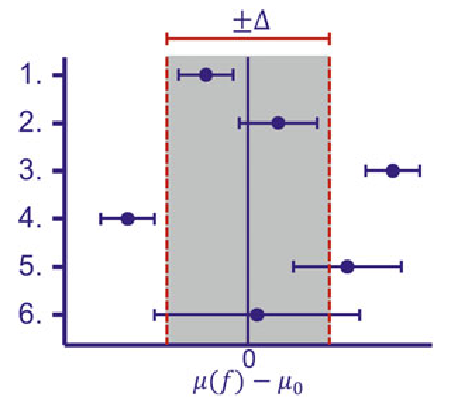
\includegraphics[
        width=\linewidth,
        height=5cm,
        keepaspectratio,
    ]{images/statistics/Equivalence-Testing.png}
    \caption*{
        Comparison between equivalence testing and traditional hypothesis testing.
        The vertical dotted lines represents the interval $[-\Delta, \Delta]$ and the vertical solid line represents the difference $\mu( f ) - \mu_0 = 0$. 
        The horizontal x-axis represents the difference $\mu( f ) - \mu_0$ and each dot in the figure represents an estimate of this difference. 
        The horizontal lines through the dots represent the $1 - 2\alpha$ confidence intervals.
        \cite{statistics/book/Statistics-for-Data-Scientists/Maurits-Kaptein}
    }
\end{figure}

    \item Equivalence testing $H_0 : \dabs{\mu( f ) - \mu_0} > \Delta$ against $H_a : \dabs{\mu( f ) - \mu_0} \leq \Delta$ is really different in concept from traditional hypothesis testing $H_0 : \mu( f ) = \mu_0$ against $H_a : \mu( f ) \neq \mu_0 $.
    \hfill \cite{statistics/book/Statistics-for-Data-Scientists/Maurits-Kaptein}
    \begin{enumerate}
        \item The $1 - 2\alpha$ confidence interval fall completely within $[-\Delta, \Delta]$, which means that the null hypothesis $H_0 : |\mu( f ) - \mu_0| > \Delta$ is being rejected. 
        It is not completely clear whether $H_0 : \mu( f ) = \mu_0$ is being rejected, since this can only be established if the $1 - \alpha$ confidence interval has been applied. 
        If we assume that this $1 - \alpha$ interval would fit within $[-\Delta, 0]$, the null hypothesis $H_0 : \mu( f ) = \mu_0$ would also be rejected. 
        This is a setting that we described earlier for large datasets, where the traditional hypothesis can be rejected for irrelevant differences.
        \hfill \cite{statistics/book/Statistics-for-Data-Scientists/Maurits-Kaptein}

        \item The null hypothesis $H_0 : |\mu( f ) - \mu_0| > \Delta$ for equivalence is being rejected, indicating that the population mean $\mu( f )$ is equivalent to $\mu_0 $. 
        The traditional hypothesis $H_0 : \mu( f ) = \mu_0$ is not being rejected, which implies that there is not enough evidence to believe that the population mean $\mu( f )$ is different from $\mu_0 $. 
        This means that both conclusions seem to coincide, although this does not imply that $\mu( f ) = \mu_0 $.
        \hfill \cite{statistics/book/Statistics-for-Data-Scientists/Maurits-Kaptein}

        \item The traditional null hypothesis is being rejected (assuming that the $95\%$ confidence interval would not contain zero) and equivalence cannot be claimed. 
        Thus both approaches seem to have similar conclusions: $\mu( f )$ is different and not equivalent to $\mu_0 $.
        \hfill \cite{statistics/book/Statistics-for-Data-Scientists/Maurits-Kaptein}

        \item This is the same as in the previous setting, although the results lie on the other side of the vertical line $\mu( f ) = \mu_0 $.
        \hfill \cite{statistics/book/Statistics-for-Data-Scientists/Maurits-Kaptein}

        \item The fact that one side of the confidence interval is contained in the interval $[-\Delta, \Delta]$ does not change the conclusions.
        \hfill \cite{statistics/book/Statistics-for-Data-Scientists/Maurits-Kaptein}

        \item Here we cannot demonstrate equivalence, but we cannot reject the traditional null hypothesis either. 
        Thus on the one hand there is not enough evidence to reject $\mu( f ) = \mu_0 $, but there is not enough evidence either to reject that $\dabs{\mu( f ) - \mu_0} > \Delta$.
        This seems contradictory, but it is probably an issue of a lack of information, since the $90\%$ confidence interval is too wide.
        \hfill \cite{statistics/book/Statistics-for-Data-Scientists/Maurits-Kaptein}
    \end{enumerate}

    \item The non-inferiority hypotheses look somewhat similar to the one-sided hypotheses, but they are not.
    In the traditional hypothesis testing format we would investigate the null hypothesis $H_0 : \mu_{N ew} \leq \mu_{Old}$ against $H_a : \mu_{N ew} > \mu_{Old}$ , assuming that a higher mean is a better clinical outcome.
    \hfill \cite{statistics/book/Statistics-for-Data-Scientists/Maurits-Kaptein}

    \item The collected data (typically through a randomized controlled clinical trial) would then have to demonstrate that the null hypothesis is rejected. 
    Thus the new treatment must demonstrate \textbf{superiority}. 
    \hfill \cite{statistics/book/Statistics-for-Data-Scientists/Maurits-Kaptein}

    \item Often new treatments are not (much) better in their clinical outcome, but they bring a secondary benefit. 
    For instance, the new treatment is much less invasive. 
    Superiority is then difficult to demonstrate. 
    Instead, we would like to show that the new treatment is not inferior to the old treatment. 
    Thus, the data must demonstrate that the new treatment is not too much worse than the old treatment: $H_a : \mu_{N ew} > \mu_{Old} - \Delta$, with $\Delta > 0$ the \textbf{non-inferiority margin}. 
    Thus, the null hypothesis becomes $H_0 : \mu_{N ew} \leq \mu_{Old} - \Delta$. 
    If this null hypothesis cannot be rejected, the new treatment is assumed inferior to the old treatment, since non-inferiority could not be proven.
    \hfill \cite{statistics/book/Statistics-for-Data-Scientists/Maurits-Kaptein}
\end{enumerate}

















